\documentclass[ebook,oneside]{memoir}

\usepackage[T1]{fontenc} % The font encoding
\usepackage[utf8]{inputenc} % The input encoding
\usepackage[USenglish]{babel} % For explicitly specifying the hyphenation rules
\usepackage[hidelinks,pdfa]{hyperref} % For clickable links
\usepackage{bookmark} % For `\bookmarksetup{startatroot}`
\usepackage[style=authoryear]{biblatex} % For citations and references
\usepackage{imakeidx} % For the index
\usepackage{microtype} % For micro-typography
\usepackage{pdfpages} % For the cover page
\usepackage[sfdefault,mono=false]{libertine} % The Linux Libertine and Biolinum typefaces
\usepackage{inconsolata} % The Inconsolata typeface

% Load the references.
\addbibresource{references.bib}

% Set up the index.
\makeindex[intoc]

\title{Syntax, Semantics, and Types}
\author{Stephan Boyer}
\date{}

\begin{document}
  % A Git commit hash
\newcommand\commit[1]{\texttt{#1}}


  \frontmatter

  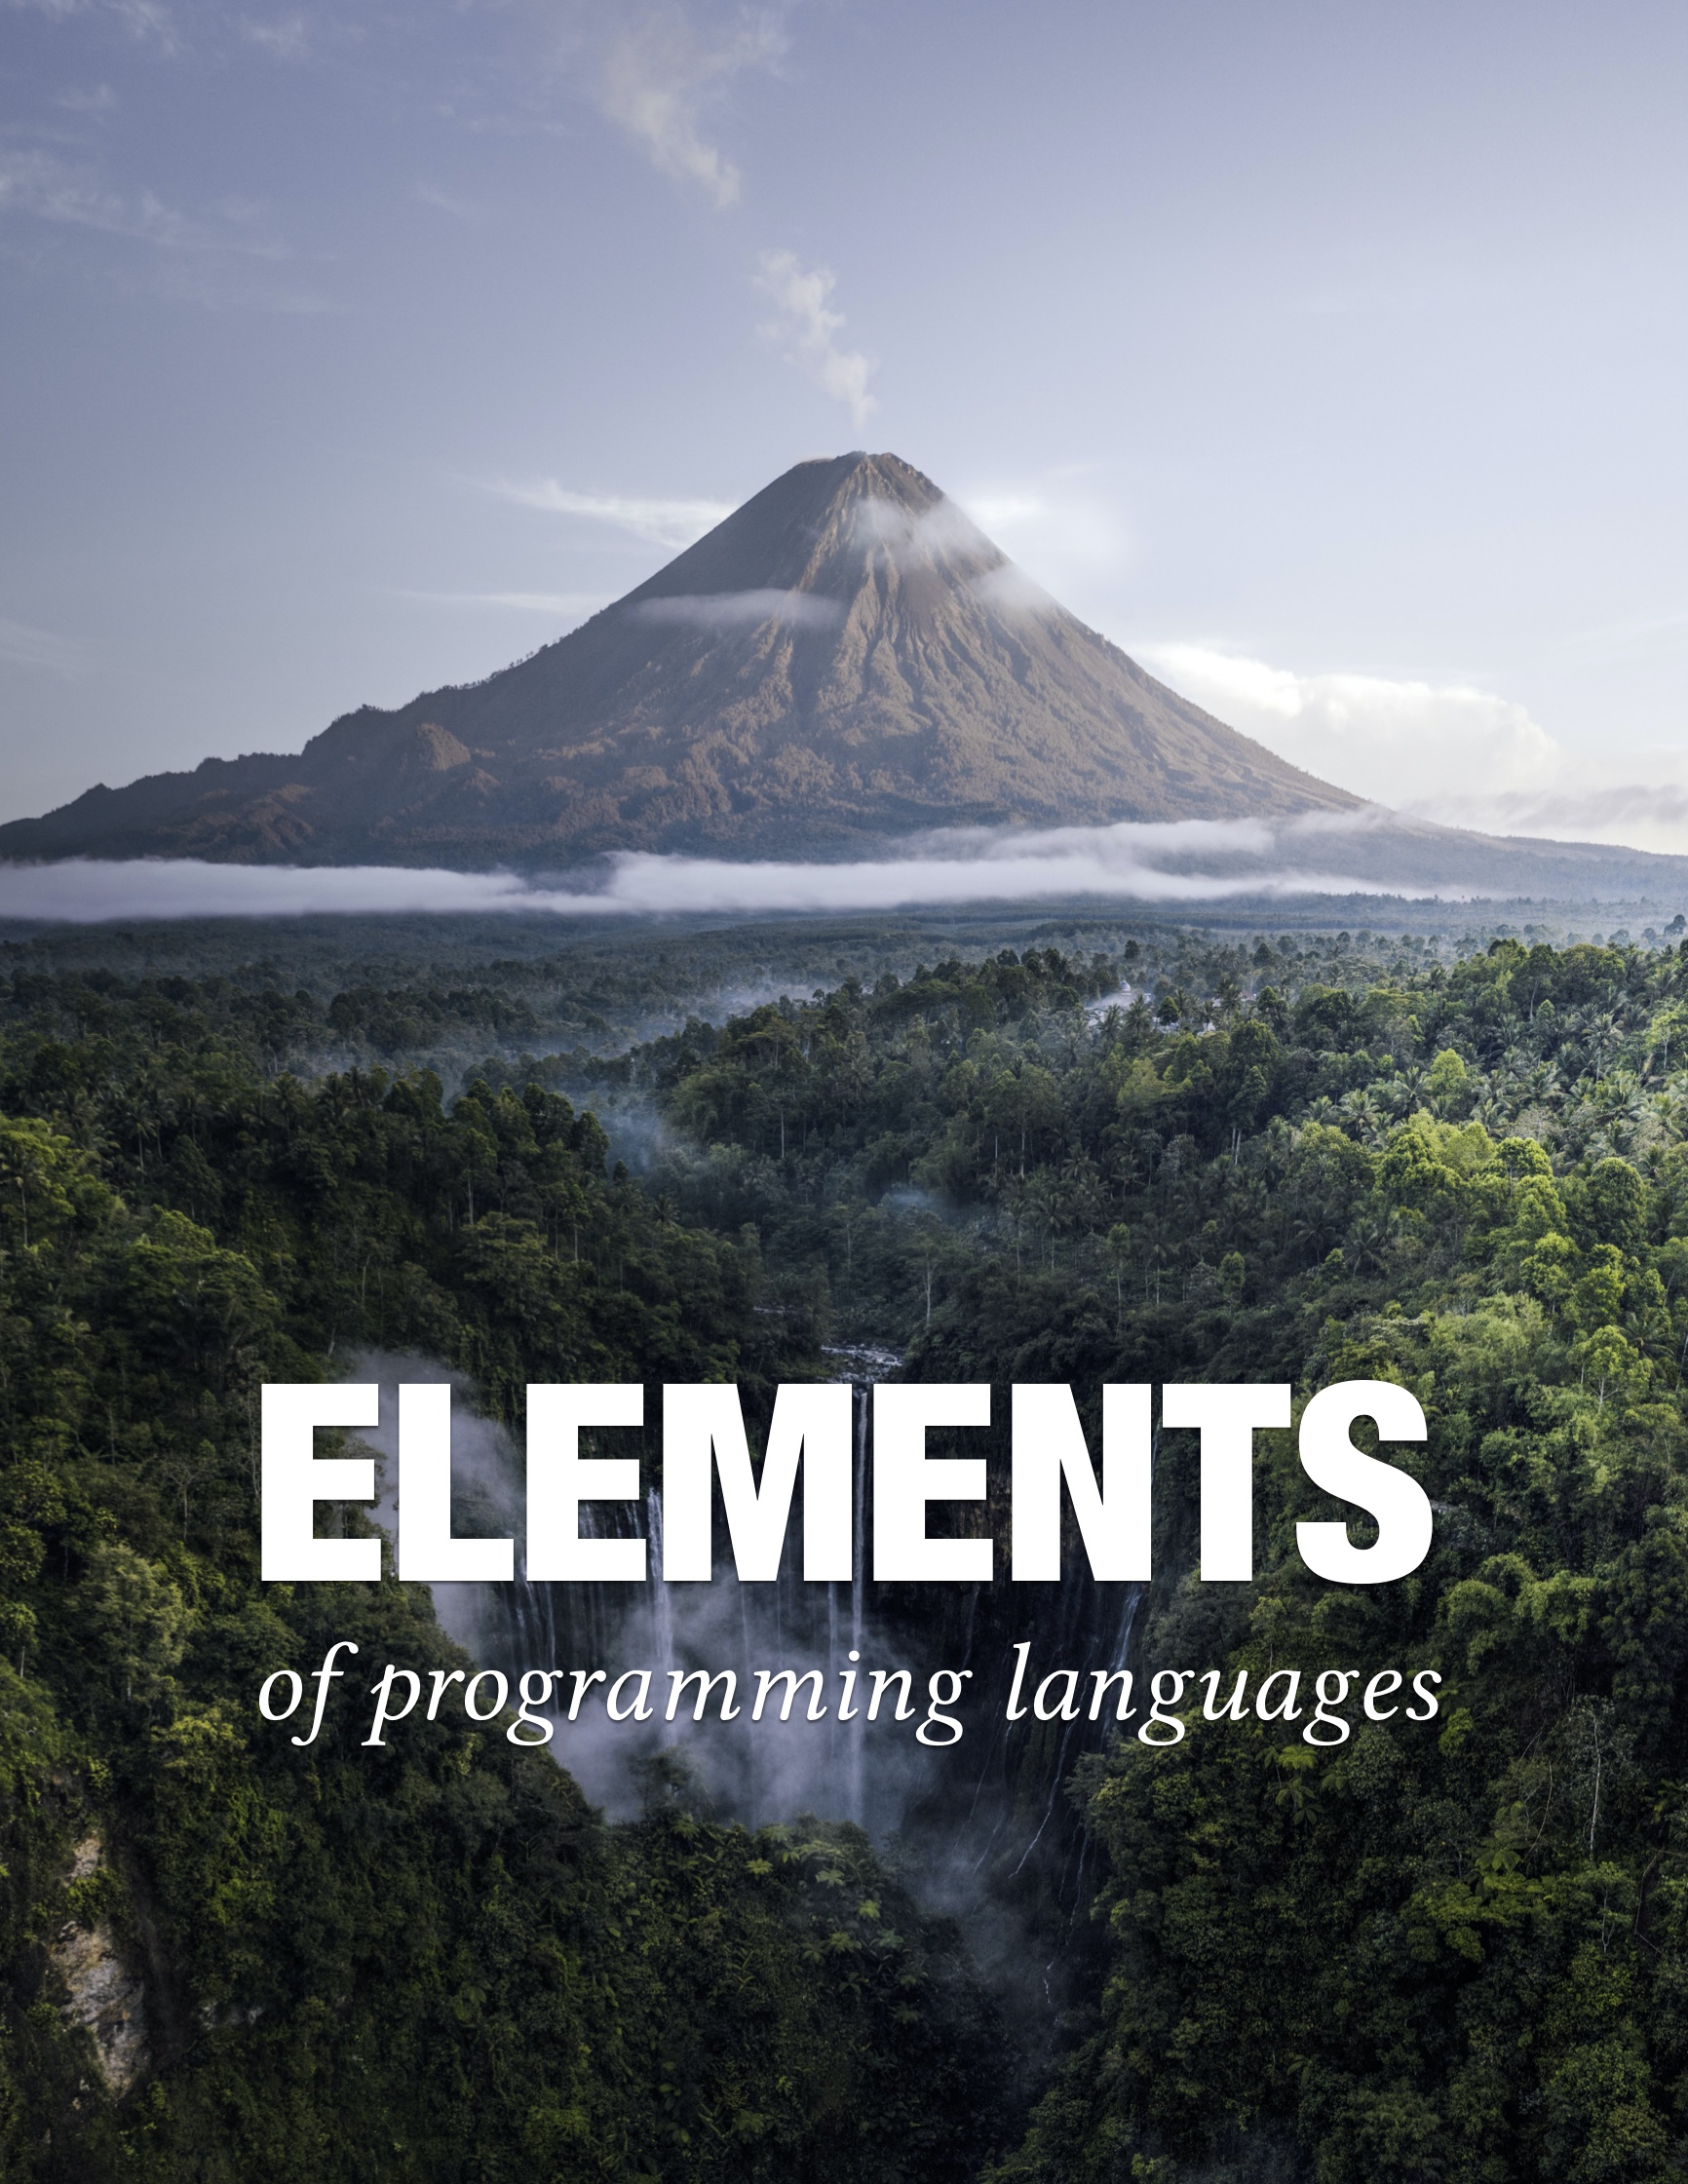
\includepdf{cover}

  \pagebreak
  \hspace{0pt}
  \vfill
    \begin{center}
      Copyright \copyright{} \the\year{} Stephan Boyer. All rights reserved.
    \end{center}
  \vfill
  \hspace{0pt}
  \pagebreak

  \chapter{Preface}

  This book is an invitation to programming language theory. It explains the mathematical devices used by researchers to formally specify programming languages, prove properties about them, and reason about programs written in them. From a bird's eye view, the three topics of this book are \emph{syntax}, \emph{semantics}, and \emph{types}. To keep the scope of the book manageable, implementation concerns such as optimization and garbage collection are not covered.

  \section*{Audience}

  \section*{Goals}

  \section*{Prerequisites}

    This text is intended to be reasonably self-contained, but the reader is expected to have a certain mathematical literacy.

    A naive understanding of the concept of \emph{set} is assumed, but no formal treatment (e.g., Zermelo--Fraenkel set theory) will be needed. The reader should be familiar with the basic operations on sets, such as union. Be sure to avoid conflating the mathematical concept of set with the abstract data type known as set. The former, which we will use extensively in this book, may be finite or infinite, whereas the latter is typically restricted to be finite.

    The reader is not assumed to know any category theory. Category theory will make an appearance, but the relevant concepts will be introduced as needed.

    These are modest prerequisites for a text on programming language theory, and perhaps that is one of the selling points for this book. In particular, it is hoped that both computer science students and professional programmers will be able to read and understand this book.

  \section*{Acknowledgements}

    The author's first formal introduction to programming language theory was \textcite{tapl}.

    The image featured on the cover depicts the Tumpak Sewu Waterfalls and the Semeru volcano in East Java, Indonesia. The photograph was captured by Filippo Cesarini and made available under the Creative Commons Zero license.

  \section*{Version}

    \input{version}


  \cleardoublepage
  \tableofcontents

  \mainmatter

  % Set the chapter heading style.
  \chapterstyle{bianchi}

  \part{Syntax}

    \chapter{Languages and grammars}

      A \emph{language}\index{language} is a set of strings.

    \chapter{Parsing}

      \section{Top-down parsing}

      \section{Bottom-up parsing}

    \chapter{Variable substitution}

  \part{Semantics}

    \chapter{Operational semantics}

      \section{Small-step operational semantics}

      \section{Big-step operational semantics}

    \chapter{Denotational semantics}

    \chapter{Axiomatic semantics}

    \chapter{Categorical semantics}

  \part{Types}

    \chapter{Simple types}

    \chapter{Sums and products}

    \chapter{Subtyping}

    \chapter{Parametric polymorphism}

    \chapter{Type operators}

    \chapter{Dependent types}

    \chapter{Recursive types}

    \chapter{Type inference}

  \backmatter
  \bookmarksetup{startatroot}
  \addtocontents{toc}{\vspace{\normalbaselineskip}}

  % Revert the chapter heading style.
  \chapterstyle{default}

  \printbibliography[heading=bibintoc,title=References]

  \printindex
\end{document}
